\documentclass[../../../../main.tex]{subfiles}

\begin{document}

\subsection*{第1問}

[解] $k$ を, $0$ から $9$ までの値をとる整数とする。又, $n$ を $1$ 以上の整数に拡張する。

(1) $f_p(10n+k) = f_p(k)$ だから, $n = 0, 1, \dots, 9$ でしらべれば良く,
\[
\begin{aligned}
&f_2(0) = 0, \quad f_2(1) = 1, \quad f_2(2) = 4, \quad f_2(3) = 9, \quad f_2(4) = 6, \quad f_2(5) = 5 \\
&f_2(6) = 6, \quad f_2(7) = 9, \quad f_2(8) = 4, \quad f_2(9) = 1
\end{aligned}
\]
より,
\[
0, 1, 4, 5, 6, 9
\]

(2) $n^5 - n = n(n+1)(n-1)(n^2+1)$ は 2 連続整数の積をもち, 2 で割り切れる。 $\cdots$ ①。又, 合同式の法を 5 として, $n^5 - n \equiv 0$ だから, $n^5 - n$ は 5 でも割り切れる $\cdots$ ②

①, ② から $n^5 - n$ は 10 で割り切れるので,
\[
f_5(n) = f_1(n)
\]
となる。 \quad 答

(3) $n^{100} = (n^4)^{25} \equiv n^4 \pmod{10}$ ($\because (2)$) だから, $f_4(n)$ のとりうる値をしらべれば良いが, $k = 0, 1, 2, 3, 4, 5$ に対し
\[
(10-k)^4 \equiv k^4 \pmod{10}
\]
だから, $k^4$ ($k=0, 1, 2, 3, 4, 5$) の 1 の位をしらべれば良く,
\[
f_{100}(n) = 0, 1, 5, 6
\]

\subsection*{第2問}

[解] 両端 $P(\alpha, \alpha^2)$, $Q(\beta, \beta^2)$ ($\alpha < \beta \cdots$ ①) とおく。$\overline{PQ} = \ell \iff \overline{PQ}^2 = \ell^2$ ($\because$ 各辺正) だから,
\[
\ell^2 = (\beta - \alpha)^2 + (\beta^2 - \alpha^2)^2 = (\beta - \alpha)^2 \left\{ 1 + (\beta + \alpha)^2 \right\} \quad \cdots \text{①}
\]
このもとで, $M(X,Y)$ のキセキをもとめる。
\[
X = \frac{\alpha + \beta}{2}, \quad Y = \frac{\alpha^2 + \beta^2}{2} \quad \cdots \text{②}
\]
ここで, $a = \alpha + \beta$, $b = \beta - \alpha$ とおくと, ①から
\[
\ell^2 = b^2(1+a^2) \quad \cdots \text{①'}
\]
又, $\alpha^2 + \beta^2 = \frac{1}{2}\{(\alpha+\beta)^2 + (\beta-\alpha)^2\} = \frac{1}{2}(a^2+b^2)$ だから, ②から
\[
X = \frac{a}{2}, \quad Y = \frac{a^2+b^2}{4} \quad \cdots \text{③}
\]
①'から $b^2 = \frac{\ell^2}{1+a^2}$ だから③に代入して
\[
Y = \frac{1}{4}\left( a^2 + \frac{\ell^2}{1+a^2} \right) \quad \cdots \text{④}
\]
さらに, $\alpha, \beta$ の存在条件から, $x$ の 2 次方程式 $x^2 - ax + \frac{a^2-b^2}{4} = 0$ が 2 実解を持つので,
\[
a^2 - (a^2 - b^2) > 0 \iff b^2 > 0
\]
①'から, これは常にみたされる。以上から, $a \in \mathbb{R}$ での $Y$ の $\min$ をもとめれば良い。$a^2, \ell > 0$ だから AM-GM より
\[
Y = \frac{1}{4} \left\{ 1 + a^2 + \frac{\ell^2}{1+a^2} - 1 \right\} \ge \frac{1}{4}(2\ell - 1)
\]
等号成立は $(1+a^2)^2 = \ell^2 \iff a = \pm\sqrt{\ell-1}$ の時だから, この時 $X = \pm\frac{\sqrt{\ell-1}}{2}$ ($\because$ ③)

以上から
\[
\left( \pm\frac{\sqrt{\ell-1}}{2}, \frac{2\ell-1}{4} \right)
\]

\subsection*{第3問}

下の図は線分ABの投影図であり, その各部の寸法は図の通りである。

\begin{center}
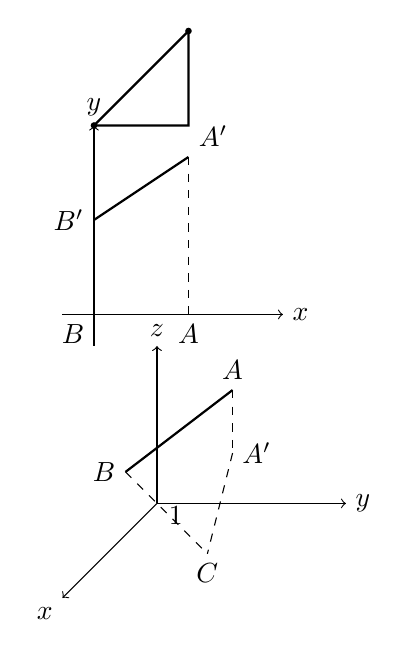
\begin{tikzpicture}[scale=0.8]
  % Projection 1 (Triangle)
  \draw[thick] (0,3) -- (1.5,3) -- (1.5,4.5) -- cycle;
  \draw[dashed] (0,3) -- (1.5,3);
  \fill (0,3) circle (1.5pt);
  \fill (1.5,4.5) circle (1.5pt);
  
  % Projection 2 (2D Axes)
  \begin{scope}[shift={(0,0)}]
    \draw[->] (-0.5,0) -- (3,0) node[right] {$x$};
    \draw[->] (0,-0.5) -- (0,3) node[above] {$y$};
    \draw[thick] (0,1.5) node[left] {$B'$} -- (1.5,2.5) node[above right] {$A'$};
    \draw[dashed] (1.5,2.5) -- (1.5,0) node[below] {$A$};
    \draw[dashed] (0,1.5) -- (0,0);
    \node[below left] at (0,0) {$B$};
  \end{scope}

  % Projection 3 (3D Axes)
  \begin{scope}[shift={(1,-3)}]
    \draw[->] (0,0) -- (3,0) node[right] {$y$};
    \draw[->] (0,0) -- (0,2.5) node[above] {$z$};
    \draw[->] (0,0) -- (-1.5,-1.5) node[below left] {$x$};
    \draw[thick] (-0.5,0.5) node[left] {$B$} -- (1.2,1.8) node[above] {$A$};
    \draw[dashed] (1.2,1.8) -- (1.2,0.8) node[right] {$A'$};
    \draw[dashed] (-0.5,0.5) -- (0.8,-0.8) node[below] {$C$};
    \draw[dashed] (1.2,0.8) -- (0.8,-0.8);
    \node at (0.3,-0.2) {$1$};
  \end{scope}
\end{tikzpicture}
\end{center}

[解] $C(X, Y, 0)$ とおく。
\[
\vec{AB} = \begin{pmatrix} 1 \\ 0 \\ -1 \end{pmatrix}, \quad \vec{AC} = \begin{pmatrix} X+1 \\ Y \\ -1 \end{pmatrix} \quad \cdots \text{(*)}
\]
まず, $\angle ACA' = \pi/6$, $|AA'| = 1$ から $|AC| = 2$ である。したがって
\[
4 = (X+1)^2 + Y^2 + 1
\]
\[
\therefore (X+1)^2 + Y^2 = 3 \quad \cdots \text{①}
\]
又 $\angle BAC = \frac{\pi}{3}$ だから,
\[
\vec{AB} \cdot \vec{AC} = \frac{1}{2} \cdot \sqrt{2} \cdot 2 = \sqrt{2}
\]
である。(*)を代入して
\[
X + 1 + 1 = \sqrt{2} \quad \therefore X = \sqrt{2} - 2 \quad \cdots \text{②}
\]
①から,
\[
Y = \pm 2^{\frac{3}{4}}
\]
だから
\[
C\left(\sqrt{2}-2, \pm 2^{\frac{3}{4}}, 0\right)
\]

\subsection*{第4問}

[解] (1)(3)から, $f'(0), g'(0)$ は有限の値を持ち,
\[
f'(0)g'(0) = -1 \quad \cdots \text{①}
\]
をみたす。ここで,
\[
\frac{ax + b f(x)}{cx + f(x)} = \frac{a x + b f(x)}{x} \cdot \frac{x}{cx + f(x)} = \frac{a + b \frac{f(x)}{x}}{c + \frac{f(x)}{x}} \xrightarrow{x \to 0} \frac{a + b f'(0)}{c + f'(0)} \quad (\because (2))
\]
同様に
\[
\frac{ax + b g(x)}{cx + g(x)} \xrightarrow{x \to 0} \frac{a + b g'(0)}{c + g'(0)}
\]
だから, (4)より,
\[
\begin{cases}
f'(0) = \dfrac{a + b f'(0)}{c + f'(0)} \\[1em]
g'(0) = \dfrac{a + b g'(0)}{c + g'(0)}
\end{cases}
\quad \therefore k^2 + ck = a + bk \quad (k = f'(0), g'(0)) \quad (\because k \neq -c)
\]
したがって, $f'(0), g'(0)$ は $x$ の 2 次方程式
\[
x^2 + (c-b)x - a = 0 \quad \cdots \text{②}
\]
の実解で, ①から, $f'(0) \neq g'(0)$ だから ($f'(0), g'(0) \in \mathbb{R}$), ②の 2 解は $x = f'(0), g'(0)$ である。したがって
\[
f'(0)g'(0) = -a
\]
だから, ①より, $a = 1$ となる。

\subsection*{第5問}

[解] 以下 $C = \cos\theta$, $S = \sin\theta$ とする。

(1)
\[
\begin{aligned}
X &= 3\cos\theta + \cos 3\theta \quad (= 4C^3) \\
Y &= 3\sin\theta + \sin 3\theta \quad (= 6S - 4S^3)
\end{aligned}
\]

(2)
\[
\begin{aligned}
\frac{dX}{d\theta} &= -3(S + \sin 3\theta) = -12S(1-S)(1+S) \\
\frac{dY}{d\theta} &= 3(C + \cos 3\theta) = 6C(2C^2 - 1)
\end{aligned}
\]
から下表をうる。
\[
\begin{array}{c|c|c|c|c|c}
\theta & 0 & \dots & \pi/4 & \dots & \pi/2 \\
\hline
X' & 0 & - & - & - & 0 \\
\hline
Y' & + & + & 0 & - & 0 \\
\hline
(X,Y) & (4,0) & \nwarrow & (\sqrt{2}, 2\sqrt{2}) & \swarrow & (0,2)
\end{array}
\]
したがって, $\max Y = 2\sqrt{2}$

(3) もとめる弧長を $L$ とする。(2)の表から
\[
\begin{aligned}
L &= \int_0^{\pi/2} \sqrt{X'^2 + Y'^2} \, d\theta \\
&= \int_0^{\pi/2} \sqrt{144 S^2 C^4 + 36 C^2 (2C^2 - 1)^2} \, d\theta \\
&= \int_0^{\pi/2} \sqrt{36 C^2} \, d\theta \\
&= \int_0^{\pi/2} 6 C \, d\theta \quad (\because C \ge 0) \\
&= 6
\end{aligned}
\]

\subsection*{第6問}

[解] Aが優勝する場合は以下のいずれか

\[
\begin{cases}
1^\circ \text{ Aの連勝 } \dots \text{ 確率 } p^3 \\
2^\circ \text{ Aの3勝1敗 } \dots {}_3\text{C}_1 p^2 \cdot q \cdot p = 3p^3 q \\
3^\circ \text{ Aの3勝2敗 } \dots {}_4\text{C}_2 p^3 \cdot q^2 = 6p^3 q^2
\end{cases}
\]
以上から
\[
P = p^3 + 3p^3 q + 6p^3 q^2 = p^3 (1 + 3q + 6q^2) \quad \cdots \text{①}
\]
同様に
\[
Q = q^3 (1 + 3p + 6p^2) \quad \cdots \text{②}
\]
ここで, $q = 1-p$ だから, ①, ②に代入して
\[
\begin{cases}
P = p^3 (6p^2 - 15p + 10) \quad \cdots \text{③} \\
Q = (1-p)^3 (1 + 3p + 6p^2) \quad \cdots \text{④}
\end{cases}
\]

(1) $p > q = 1-p$ つまり $\frac{1}{2} < p < 1$ の時, $f(p) = P - Q - p + q$ とおくと, $P+Q = 1$ から
\[
\begin{aligned}
f(p) &= 2(P-p) \\
&= 2\left(p - \frac{1}{2}\right) \cdot p \cdot (p-1) (3p^2 - 3p - 1)
\end{aligned}
\]
ここで, $\frac{1}{2} < p < 1$ から, $p - \frac{1}{2} > 0$, $p-1 < 0$, $3p^2 - 3p - 1 < 0$ だから, $f(p) > 0$。よって
\[
P - Q > p - q
\]

(2)
\[
\begin{aligned}
\frac{1}{2} f'(p) &= 30p^4 - 60p^3 + 30p^2 - 1 \\
&= 30p^2(p^2 - 2p + 1) - 1 \\
&= 30p^2(p-1)^2 - 1
\end{aligned}
\]
から, $f'(p) \ge 0 \iff p^2(p-1)^2 \ge \frac{1}{30} \iff p(1-p) \ge \frac{\sqrt{30}}{30} \quad (\because 0 < p < 1)$
\[
\iff \frac{1 - \sqrt{1 - \frac{2}{15}\sqrt{30}}}{2} \le p \le \frac{1 + \sqrt{1 - \frac{2}{15}\sqrt{30}}}{2}
\]
だから, 一部を $\alpha, \beta$ ($\alpha < \beta$) として表をつくると
\[
\begin{array}{c|c|c|c|c|c|c|c}
p & 0 & \dots & \alpha & \dots & \beta & \dots & 1 \\
\hline
f' & & - & 0 & + & 0 & - & \\
\hline
f & & \searrow & & \nearrow & & \searrow &
\end{array}
\]
したがって, $P-p$ を最大にするのは, $p = 0$ 又は $\beta$ である。ここで, (1)から $f(0) = 0$ で, $\frac{1}{2} < p$ の時 $f(p) > 0$ だから, $\beta > \frac{1}{2}$ より $f(\beta) > 0$。以上から $f(0) < f(\beta)$ だから,
もとめるのは
\[
\beta = \frac{1 + \sqrt{1 - \frac{2}{15}\sqrt{30}}}{2}
\]

(3)
\[
\begin{cases}
3 \text{回でおわる} \dots p^3 + q^3 \\
4 \text{回でおわる} \dots 3p^3 q + 3q^3 p \\
5 \text{回でおわる} \dots 6(p^3 q^2 + q^3 p^2)
\end{cases}
\]
だから
\[
\begin{aligned}
N &= 3(p^3 + q^3) + 12(p^3 q + q^3 p) + 30(p^3 q^2 + q^3 p^2) \\
&= 3(p^3 + q^3) + 12pq(p^2 + q^2) + 30p^2 q^2 \\
&= 3(p+q)(p^2 - pq + q^2) + 12pq \{ (p+q)^2 - 2pq \} + 30p^2 q^2 \\
&= 3(p^2 - pq + q^2) + 12pq(1 - 2pq) + 30p^2 q^2 \\
&= 3(1 - 2pq) + 9pq + 6p^2 q^2 = 3 + 3pq + 6p^2 q^2
\end{aligned}
\]
$t = pq$ として,
\[
\frac{dN}{dt} = 3 + 12t > 0 \quad (\because t > 0)
\]
だから, $t$ が最大の時 $N$ も最大。$t = pq = p(1-p) \le \frac{1}{4}$ (等号成立は $p = \frac{1}{2}$)
より, $N$ は $p = \frac{1}{2}$ で $\max N = \frac{33}{8}$ をとる。

\end{document}
